\ifpdf
    \graphicspath{{Appendix2/Appendix2Figs/PNG/}{Appendix2/Appendix2Figs/PDF/}{Appendix2/Appendix2Figs/}}
\else
    \graphicspath{{Appendix2/Appendix2Figs/EPS/}{Appendix2/Appendix2Figs/}}
\fi  


\section{Heuristic artefacts}
\label{app:heartefacts}

\subsection{Heuristic descriptions}\label{sect:hedescriptions}

\begin{longtable}{|p{12cm}|p{1cm}|}
%\caption{Heuristic Description}\\
\hline
\textbf{Heuristic} & \textbf{Code} \\
\hline
\endfirsthead
\multicolumn{2}{c}%
{\tablename\ \thetable\ -- \textit{Continued from previous page}} \\
\hline
\textbf{Heuristic} & \textbf{Code} \\
\hline
\endhead
%\hline 

\multicolumn{2}{r}{\textit{Continued on next page}} \\
\endfoot
\hline
\endlastfoot

INFORMATION CODING (VISUAL REPRESENTATION): The perception of information is directly dependent on the mapping of data elements to visual objects. This should be enhanced by using realistic characteristics/techniques or the use of additional symbols. \par
\textit{Example guidelines:}
\begin{itemize}
\item Are the data to visual element mappings understandable and effective?
\item Is the use of additional symbols in the representation understandable and effective? 
\item Can you get a general understanding of the underlying data values of an individual item and where the individual data item fits into the overall dataset?
\end{itemize}

& B5 \\ \hline

MINIMAL ACTIONS: Workload with respect to the number of actions necessary to accomplish a task. It is a matter of limiting as much as possible the steps users must go through.
\par
\textit{Example guidelines:}
\begin{itemize}
\item Are the number of steps required to perform a task reasonable?
\item For data entry, are currently defined default values displayed in their appropriate data fields?
\item Can the user directly go to a requested view, without having to go through intermediaries?
\end{itemize}

& E7 \\ \hline
FLEXIBILITY: Number of possible ways of achieving a given goal, means available for customisation to take into account working strategies, habits and task requirements. 
\par
\textit{Example guidelines:}
\begin{itemize}
\item Are users provided with sufficient means to control visualisation configuration?
\item Are users permitted to define, change or remove default values for settings?
\item When some displays are unnecessary, can users remove/hide them temporarily?
\item Can users change settings in any order?
\end{itemize}

& E11 \\ \hline
CONSISTENCY: Design choices are maintained in similar contexts and different when applied to different contexts.
\par
\textit{Example guidelines:}
\begin{itemize}
\item Are window titles always located in the same place?
\item Are the configuration controls consistent?
\item Are similar procedures used to perform tasks?
\item Are labels (phrasing, punctuation, placement) consistent?
\end{itemize}

& E16 \\ \hline
RECOGNITION RATHER THAN RECALL: The user should not have to memorise a lot of information to carry out tasks.
\par
\textit{Example guidelines:}
\begin{itemize}
\item Are the available user actions visible to the user?
\item Can the user perform tasks without having to recall information?
\item Can tasks be performed without referring to external documentation?
\end{itemize}

& C6 \\ \hline
SPATIAL ORGANISATION (VISUAL REPRESENTATION): User's orientation in the information space, distribution of elements in the layout, precision and legibility, efficiency in space usage and distortion of visual elements.
\par
\textit{Example guidelines:}
\begin{itemize}
\item Can I easily locate an information element in the display?
\item Are the individual elements legible?
\item Is space used efficiently in the layout?
\item Am I aware of the overall distribution of information elements in the representation?
\item Are some objects occluded by others?
\item Does the layout follow a logical organisation?
\item Do I understand how tag placement is related to the selected layout and ordering? 
\end{itemize}

& B3 \\ \hline
REMOVE THE EXTRANEOUS: minimising the distracting effect of extra information when locating information, gaining an overview, or making a comparison. 
\par
\textit{Example guidelines:}
\begin{itemize}
\item Are means provided to reduce the distracting effect of extra information when locating information?
\item Are means provided to reduce the distracting effect of extra information when gaining an overview?
\item Are means provided to reduce the distracting effect of extra information when   making a comparison?
\end{itemize}

& D10 \\ \hline
DATASET REDUCTION (INTERACTIVITY MECHANISM): Concerns the provided features for reducing a dataset, their efficiency and ease of use.
\par
\textit{Example guidelines:}
\begin{itemize}
\item Are means provided to filter/reduce a dataset?
\item Are means provided to “prune” or cut off information that may be irrelevant?
\item Are filtering mechanisms efficient and easy to use?
\end{itemize}

& B9 \\ \hline
ORIENTATION AND HELP (INTERACTIVITY MECHANISM): Functions like support to control levels of details, redo/undo of actions and representing additional information. 
\par
\textit{Example guidelines:}
\begin{itemize}
\item Are means provided to control levels of detail?
\item Are means provided to redo/undo user actions?
\item Is requested additional information represented, or accessible?
\end{itemize}

& B7 \\ \hline
PROMPTING: Refers to the means available in order to guide the users towards making specific actions and means that help users to know the alternatives when several actions are possible depending on the contexts. Prompting also concerns status information, that is information about the actual state or context of the system, as well as information concerning help facilities and their accessibility.
\par
\textit{Example guidelines:}
\begin{itemize}
\item Are users aware of valid values for interface options?
\item Are measurement units displayed for data entry?
\item Is status information displayed?
\item Are labels provided for all fields?
\item Are cues provided on the acceptable length of data entries?
\item Are titles provided for each window?
\item Is on-line help and guidance provided?
\end{itemize}

& E1 \\ 
%\hline
%\hline
%\end{tabular}
\label{tab:heuristics}
\end{longtable}

\subsection{Heuristic checklist}\label{sect:checklist}

\begin{figure}[!htb]
	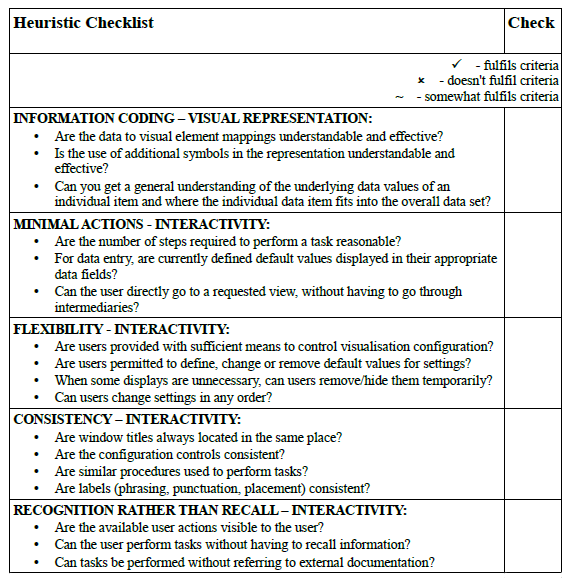
\includegraphics{checklist1.png}
\end{figure}

\begin{figure}[!htb]
\begin{subfigure}{\textwidth}
	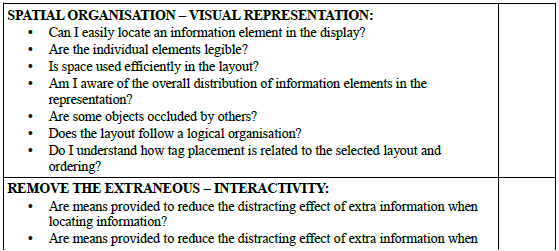
\includegraphics{checklist2.png}
\end{subfigure}
\begin{subfigure}{\textwidth}
	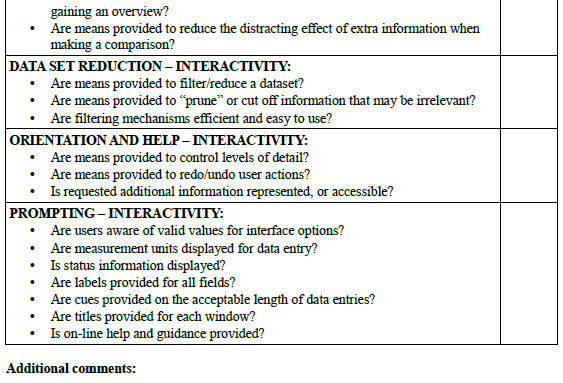
\includegraphics{checklist3.png}
\end{subfigure}
\end{figure}
%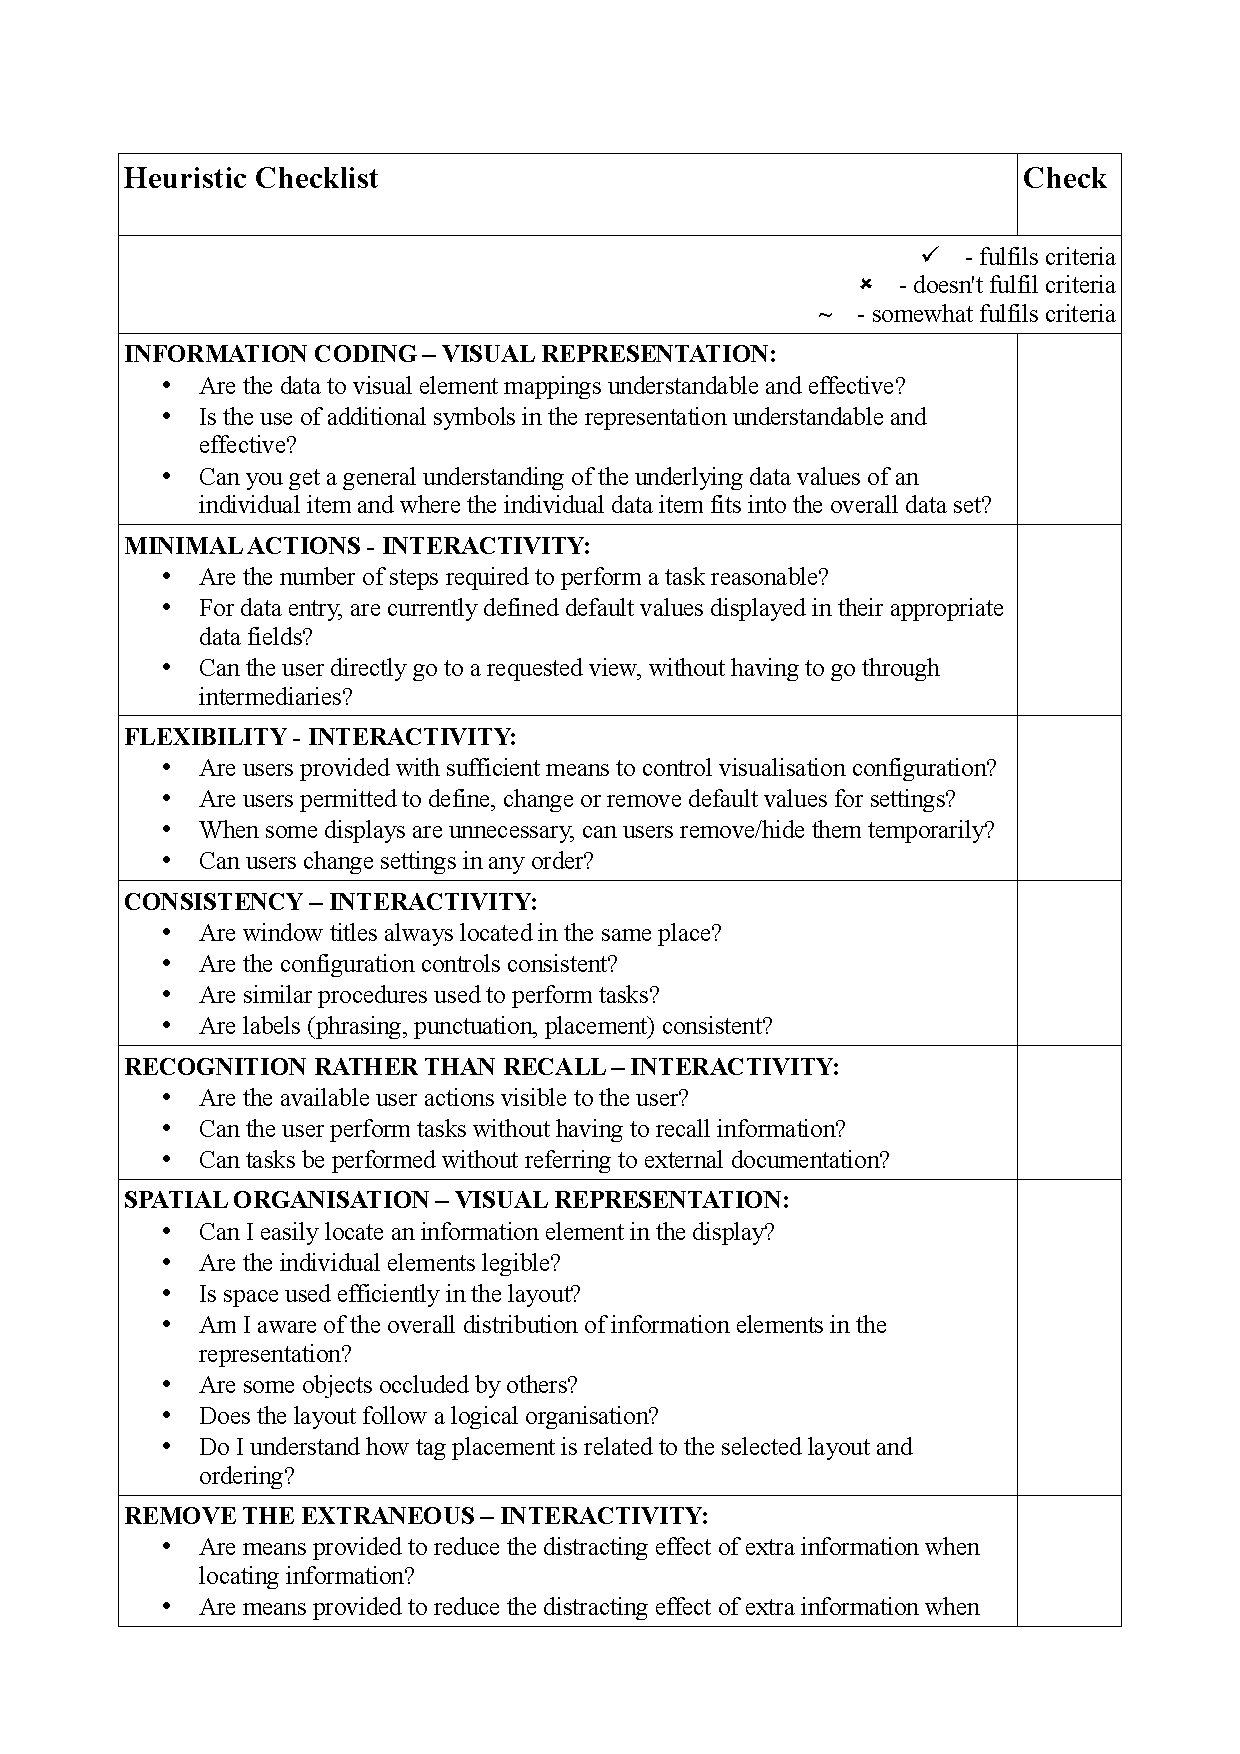
\includepdf[pages=-]{HeuristicChecklist.pdf}

\newpage
\subsection{Typical usage patterns}\label{sect:usagepatterns}

Sample tasks for exploration of a dataset.

\paragraph{Set-up of mappings}
Note that mappings can be either NUMERICAL or ALPHABETICAL. 

\begin{enumerate}
\item Map tag text to a variable e.g. `Baby name popularity' dataset map tag text to variable 'Name'.
\item Map order (layout) to a variable e.g. `US popularity'. The data is laid out from smallest value to largest OR from largest value to smallest if `reverse order' is checked. Choose a layout algorithm of typewriter or spiral. Use step layout to see how/where individual tag elements are placed.
\item Map font size to a variable e.g. `US popularity'. The smallest font size will be mapped to smallest data values and largest font size to the largest data values.
\item Map colour to a variable e.g. `NZ popularity'. The `from' colour will be mapped to smallest data values and 'to' colour to the largest data values. 
\item Press `Update/reset cloud' to produce a cloud.
\end{enumerate}


\paragraph{Interacting with the data and filtering information}

\begin{itemize}
\item Filter tags on a delimiter (mouse wheel scroll) e.g. filter out package names in a class
\item Filter tag labels that are too long (mouse wheel scroll) e.g. filter agile story labels to only 6 characters
\item Remove tags temporarily from dataset e.g. remove runners from a particular club
\item Filter tags from a dataset, keeping them in view (dynamic filters) e.g. tag the tag colour of runners from a particular club
\item When there are too many tags to display in the window, some of the smaller ones will be displayed with a + symbol
\item Make a new cloud from a selected subset of tags
\item Set the tag colour to be displayed in the background
\item Compare tags by selecting and dragging next to one another
\end{itemize}


\paragraph{Exploring data and generating hypotheses}

\begin{itemize}
\item Identify correlations in the data e.g. baby names that are popular in the NZ appear correlated with popular baby names in the US
\item Outlier identification e.g. the estimate for this agile story is much higher than the other stories
\item Identify clusters of data with similar characteristics e.g. runners from this club have a lower score
\item Locate a particular data element e.g. find the most popular baby name in the US
\item Compare multiple data elements e.g. which baby name is more popular, `Shane' or `Antonio'
\item Identify the distribution of the data e.g. most users have a low average number of hours to fix a software bug
\end{itemize}

\newpage
\subsection{Usability issues found linked to heuristics}\label{sect:heuristicresults}

\begin{table*}[!htb]
\centering
\caption{\textit{Mapping Selection/Cloud Creation}}
\begin{tabular}{|p{4cm}|p{8cm}|x{2cm}|} \hline
\textbf{Heuristic}&\textbf{Issue}&\textbf{Severity}\\ \hline
E7 (minimal actions)\par E1 (prompting) & Need overview of data immediately when first open a dataset & 3 \\ \hline
E1 (prompting) & Mapping font size to text (alphabetical) isn't helpful & 3 \\ \hline
E1 (prompting) & Figuring out what mappings to use to initially very difficult & 5 \\ \hline
E1 (prompting) & There are too many variables to play with. Need to reduce at the start and pair up e.g. size/order. I cannot be sure if there is a relationship in the data or I just haven't found it yet. (Rephrased --- I need guidance towards taking an appropriate  action specific to my task). & 4 \\ \hline
E16 (consistency)\par D10 (remove the\par extraneous)\par E7 (minimal actions) & Require the mappings to be reversed if data hasn't been filtered correctly, like what you can do with order (Rephrased --- I shouldn't have to have to edit my source file to reverse data). & 3 \\ \hline
E7 (minimal actions) & Having to click update/reset after each mapping change & 2\\
\hline\end{tabular}
\label{table:mappingselection}
\end{table*}

\begin{table*}[!htb]
\centering
\caption{\textit{Static and Dynamic Filtering}}
\begin{tabular}{|p{4cm}|p{8cm}|x{2cm}|} \hline
\textbf{Heuristic}&\textbf{Issue}&\textbf{Severity}\\ \hline
E7 (minimal actions)\par B9 (dataset reduction) & It is is easy to forget the filter check box & 3 \\ \hline
B9 (dataset reduction) & It is not obvious how the dynamic filter worked and the red, green, blue colours were confusing & 2 \\ \hline
B9 (dataset reduction)\par E16 (prompting)\par E7 (minimal actions) & Don't reset mouse wheel when click update/reset cloud. Also I didn't know how to use it until explained & 2 \\
\hline\end{tabular}
\label{table:filtering}
\end{table*}

\begin{table*}[!htb]
\centering
\caption{\textit{Information Coding and Spatial Organisation}}
\begin{tabular}{|p{4cm}|p{8cm}|x{2cm}|} \hline
\textbf{Heuristic}&\textbf{Issue}&\textbf{Severity}\\ \hline
B5 (information coding)& One colour per class when mapping data to colours (colour legend) & 2 \\ \hline
B3 (spatial organisation)& Spiral is easier to see patches of clubs with high scores, don't get the disjoint at the end of each row in typewriter layout & 3 \\
\hline\end{tabular}
\label{table:informationcoding}
\end{table*}

% ------------------------------------------------------------------------

%%% Local Variables: 
%%% mode: latex
%%% TeX-master: "../thesis"
%%% End: 
